\section{Experiments}
\begin{figure*}
  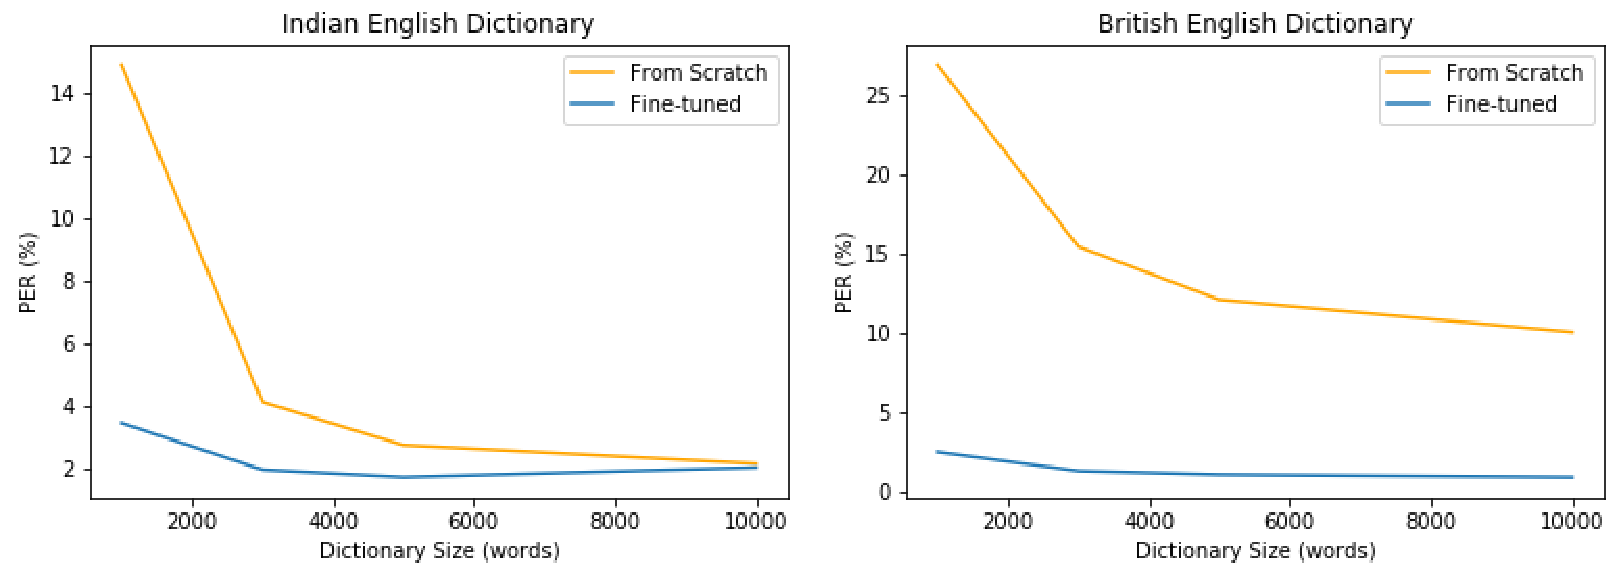
\includegraphics[width=\linewidth]{figures/g2p_results.pdf}
   \caption{Comparing training from scratch and transfer learning as dictionary size increases.  (Left) Results for the Indian English dictionary.  (Right) Results for the British English dictionary.}
   \label{fig:britishresults}
\end{figure*}

\subsection{Dataset Creation} 
We use publicly available dictionaries to create our training and test datasets. We also avoid data automatically scraped from websites like Wikitionary\footnote{\url{https://en.wiktionary.org/wiki/Wiktionary}}, as such data is \emph{noisier} and less reliable~\cite{schlippe2010wiktionary}. We use CMUDict\cite{weide2005carnegie} and Indian English dictionaries from the CMUSphinx project. We also use Britphone dictionary by Jose Llarena\footnote{\url{https://github.com/JoseLlarena/Britfone}} for our British English (Received Pronunciation) dictionary. For every word with more than one pronunciation, that is, specifically not marked for a certain part of speech (in CMUDict's homonyms list), we take the first appearance of the word as its pronunciation. We tackle the G2P problem with full utterances to their phonetic transcriptions as a sequence-to-sequence problem, not as individual words but as entire sentences. To generate our training data, we take sentences from the LibriTTS\cite{zen2019libritts} dataset and split sentences for training/dev/test sets accordingly. We use the phoneme dictionaries to generate ground-truth phonetic sequences that correspond to the original sentences.

To make our training/test distributions more similar to real world scenarios, where the dictionary used for training has limited words compared to all sentences, we limit the number of words the dictionary has for training data, and filter out sentences that have any words not in this limited dictionary data. For testing our models, all words in the dictionary are used to generate the data, filtering out sentences that have words not in the dictionary.

To ensure that even extremely small subsets of large dictionaries contain common words such as ``the'' or ``of'', we compute the frequency of every word in the training set, and add words to the dictionaries based on their frequency. This helps build realistic \emph{pseudo-small} dictionaries from larger dictionaries. This is done because when dictionary for new dialect is built, the most common words in that dialect retain higher priority and increase the sentence coverage of that dictionary.

The 3\% shortest and 3\% longest sentences are filtered out of the training, validation, and test sets. This is done because the shortest sentences are single word utterances that often have more punctuation than letters. The longest sentences are filtered out to accommodate the maximum sequence length of the transformer model used, as extremely long sequences are computationally and memory intensive.
% 
\subsection{Transfer Learning for English Dialects.} 
We generate dictionaries of 4 sizes for training: 1K words, 3K words, 5K words, and 10K words.  As the British English dictionary has 15221 words not counting alternate pronunciations, we do not train with any larger vocabulary.  For each dialect, a model is trained from scratch on each dictionary size, and a model is fine-tuned on each dictionary size.  In total, we train 16 different models for comparison.

We pretrain a model on data generated by the American English (CMUDict) dictionary for 100 epochs, selecting the lowest validation loss model as our checkpoint. We initialize our \emph{transfer-learned} models with the pretrained checkpoint.  We replace the output layers to match the new phonetic output size, and the whole model is fine-tuned for 25 epochs on the target dialect data. The checkpoint with the best validation loss is selected for testing. We also train the same model from scratch for 50 epochs to compare the utility of transfer learning.  At the end of every epochs, the validation loss is calculated on the dev set, and the final checkpoint is chosen based on lowest validation loss.

The models we train overfit to the data with small dictionary sizes, both from scratch and transfer learned, requiring validation loss checkpoint selection.  However, as the dictionary size increases, the overfitting decreases, and the Indian English models for 10K are likely undertrained with the standard number of epochs used for all models. The transfer learned models are able to achieve significantly lower validation and training loss before starting to overfit, this is more true for smaller dictionary sizes and the British English data, where the dictionary was able to generate far fewer sentences than the Indian English dictionary was.  For example, with a dictionary size of 5K words, the British English dictionary generated almost 9K training sentence-phoneme pairs, while the Indian English dictionary generated 87K sentence-phoneme pairs.  This discrepancy in data scale is likely why the Indian English from scratch models start to attain performance competitive with pretrained models at 10K words, while the British English from scratch models are still an order of magnitude worse in PER compared to the fine-tuned models.

\subsection{Results}
Our results show that transfer learning is effective means for building robust G2P models on dialects with extremely limited data. 
\\
\\
\textbf{British English Dictionary} The British English dictionary results shows this most effectively, as the dictionary size is inflated due to differing spellings across American and British English, e.g., ``color'' vs ``colour''. Even with this inflation of words, the fine-tuned British English dictionary of 1K words results in a low PER of only 2.469\%, see Figure~\ref{fig:britishresults}, right. As the full British English dictionary only has 15211 words when counting unique words, the improvement of the fine-tuned model is significant, as unlike CMUDict and the Indian English dictionary, that are large and have vocabularies of over 100K words. We note that the British English dictionary itself is not sufficient to train a robust G2P model from scratch, since, even with a training dictionary of size 10K words, the \emph{from scratch} model reaches 10.017\% PER, and the fine-tuned model achieves 0.875\% PER. The British English model suffers from a lower amount of training data per dictionary size as compared to the Indian English data, likely due to the LibriTTS dataset containing sentences more similar to the American English dialect than the British English dialect.
\\
\\
\textbf{Indian English Dictionary.} The Indian English dictionary results show that dictionaries without multiple spellings of the same word can have the gap quickly narrowed as the training data rapidly increases with dictionary size. With a 10K word dictionary for Indian English, a significant amount of training data is generated (\textgreater 100K training sentence-phoneme pairs). Models trained on larger amounts of data may benefit from more training epochs than were, in our experiments. The Indian English model fine-tuned on the 10K word dictionary data with the best validation loss came from the last epoch of training, while more training may have improved its performance. This explains its anomalous increase in PER compared to the other results from the Indian and British dictionaries. Despite the likely under-training of the models with large dictionary sizes for Indian English, the fine-tuned model's results (2.039\% PER) still improves upon the PER of the from scratch model (2.166\% PER) with half the training steps, making it much more computationally efficient, Figure~\ref{fig:britishresults}, left.


\subsection{Edge Cases}

As described in the Section~\ref{sec:intro}, dictionary-based G2P systems can run into edge cases, that can lead to inaccuracies. The main cause are: new words with confusing pronunciation, long words that cause the fallback neural network to fail, and 3) words that are misspelled and alternate spellings of the same word. Such edge cases can cause G2P to fail, and subsequent TTS is incorrect.

An example of the various edge cases is the poem \emph{Jabberwocky by Lewis Carroll}\footnote{\url{https://www.poetryfoundation.org/poems/42916/jabberwocky}}, which is full of invented words that lack meaning. These words pronunciation are guessed by the readers, although the rhyming structure of the poem does provide some clues. Our pretrained, and transfer-learned models are more capable of pronouncing this poem than dictionary systems that fail on words not in their vocabulary. We also note that some of the ``from scratch'' models have trouble with this poem, and the dictionaries used to train these systems would fail with invented lexicon of this poem. For example, for the original sentence:

\emph{\textcolor{blue}{``Beware the Jubjub bird, and shun The frumious Bandersnatch!''}}
\\
\\
\textit{British English 10K words -- Fine-tuned model} gives:

\textcolor{blue}{\textipa{b I w " E @ D " i : d Z " 5 b b " 3 : d , @ n d S " 5 n D " i : f \*r " u : m I @ s b " \ae n d @ z n " \ae tS !}}
\\
The fine-tuned model makes mistakes, for example, the word ``jubjub'' is translated to pronunciation as just \textipa{d Z " 5 b}, or ``jub''; a failure to repeat the sound again as the original word calls for.
\\
\\
\textit{British English 10K words -- From scratch model} gives:

\textcolor{blue}{\textipa{b j " u : D " E @ d Z " u : t b " 3 : d , \*r " 5 n d D @ S " a U n b l " A : f I s m @ \*r " e I S @ n s t s!}}
\\
In this phonetic transcript, the only word that can be identified with unambiguously correct pronunciation is the word ``bird'', and is translated to \textipa{[b " 3 : d]}. In this case, rest of the phonetic pronunciation is unclear, and only vaguely resembles the words the model was given. We also compare the longest word between the two models, \emph{\textcolor{blue}{bandersnatch}}. As it is the last word, it takes the last 9 phonemes from the models:
\begin{enumerate}
    \item[-] Fine-tuned model: \textcolor{blue}{\textipa{b " \ae n d @ z n " \ae t S}}
    \item[-] From scratch model: \textcolor{blue}{\textipa{@ \*r " e I S @ n s t s}}
    \item[-] Ground Truth pronunciation\footnote{\url{https://www.collinsdictionary.com/dictionary/english/bandersnatch}}:  \textcolor{blue}{\textipa{'" b \ae n d @ "" s n \ae t S}} 
\end{enumerate}
% 
% and found just before a comma as in the original sentence.
% 
% 
% 
% \subsection{Dataset}
% Many G2P systems use proprietary data that is unavailable to the public.  In our work, we use only publicly available dictionaries to create our training and testing data.  We also avoid using data automatically scraped from websites like Wikitionary, as such data is noisier and less reliable. We use the CMUDict dictionary and the Indian English dictionary from the CMUSphinx project.  We also use the Britphone dictionary by Jose Llarena for our British English (Received Pronunciation) dictionary.  For every word with more than one pronunciation that is not specifically marked for a certain part of speech as in CMUDict's homonyms list, we take the first appearance of a word as its pronunciation.  The G2P problem we tackle is full utterances to their phonetic transcriptions, a sequence-to-sequence problem, not individual words but entire sentences.  To generate our training data, we take sentences from the LibriTTS train sets as training sentences, development sets as dev/validation sentences, test sets as test sentences, and use the dictionaries to generate ground-truth phonetic sequences that correspond to the original sentences.

% To make our train/test distributions more similar to real-world scenarios where the dictionary used for training has limited words compared to all sentences, we limit the number of words the dictionary has for training data, and filter out sentences that have any words not in this limited dictionary data.  For testing our models, all words in the dictionary are used to generate data, again filtering out sentences that have words not in the dictionary.

% To ensure that even extremely small subsets of large dictionaries contain common words such as ``the'' or ``of'', we compute the frequency of every word in the training set, and add words to the dictionaries based on their frequency.  This is realistic for building pseudo-small dictionaries from large dictionaries, as when building a dictionary for a new dialect, the most common words in that dialect would be the highest priority words to quickly increase the sentence coverage of that dictionary.

% The 3\% shortest and 3\% longest sentences are filtered out of the training, validation, and testing set.  This is because the shortest sentences are single-word utterances that often have more punctuation than graphemes.  The longest sentences are filtered out to accommodate the max sequence length of the transformer model used, as extremely long sequences are computationally and memory intensive.
% \subsection{Transfer Learning for English Dialects}
% We initialize our transfer-learned models with a checkpoint pre-trained on American English (CMUDict) for 100 epochs, the checkpoint is from the epoch with the lowest validation loss.  The output layers are then replaced to match the new phonetic output size, and the whole model is fine-tuned for 25 epochs on the target dialect data, and the checkpoint with the best validation loss is used for testing.

% We also train the same model from scratch for 50 epochs to compare the utility of transfer-learning, again choosing the checkpoint with the lowest validation loss for testing.
% \begin{figure}[hbt!]
%   \includegraphics[width=\linewidth]{figures/british_dictionary_results.png}
%   \caption{Results for the British English dictionary, comparing training from scratch with transfer learning as dictionary size increases.}
%   \label{fig:britishresults}
% \end{figure}

% \begin{figure}[hbt!]
%   \includegraphics[width=\linewidth]{figures/indian_dictionary_results.png}
%   \caption{Results for the Indian English dictionary, comparing training from scratch with transfer learning as dictionary size increases.}
%   \label{fig:britishresults}
% \end{figure}